\documentclass[11pt,a4paper]{article}

\usepackage[margin=1in]{geometry}
\usepackage{booktabs}
\usepackage{graphicx}
\usepackage{amsmath}
\usepackage{xcolor}
\usepackage{hyperref}

\hypersetup{
    colorlinks=true,
    urlcolor=blue!60!black,
    linkcolor=black
}

\title{\textbf{CS6886 -- Assignment 2: MobileNet-v2 Compression}\\[2mm]}
\author{Madhav Bhardwaj \quad \texttt{CS23B035}}
\date{\today}

\begin{document}

\maketitle

\noindent
\textbf{Repository:}
\url{https://github.com/Madhav1729/cs6886-a2-mobilenetv2-compression} \\

\textbf{W\&B Dashboard:}
\url{https://wandb.ai/cs23b035-iit-madras/cs6886-a2-mobilenetv2}

\vspace{4mm}

%======================================================================

\section{Baseline Training}

%======================================================================

\subsection{Data Pipeline}

We used the CIFAR-10 dataset, which has 50,000 training images and 10,000 test images. Table~\ref{tab:transforms} shows how we prepare the images.

\begin{table}[ht]
\centering
\begin{tabular}{@{}lll@{}}
\toprule
\textbf{Step} & \textbf{Train} & \textbf{Test} \\
\midrule
1 & \texttt{RandomCrop(32, padding=4, padding\_mode='reflect')} & --- \\
2 & \texttt{RandomHorizontalFlip(p=0.5)} & --- \\
3 & \texttt{Resize(160, interpolation=BICUBIC)} & \texttt{Resize(160, BICUBIC)} \\
4 & \texttt{ToTensor()} & \texttt{ToTensor()} \\
5 & \texttt{Normalize(ImageNet stats)} & \texttt{Normalize(ImageNet stats)} \\
\bottomrule
\end{tabular}
\caption{Data preprocessing steps.}
\label{tab:transforms}
\end{table}

We made two main choices here:

\begin{itemize}

\item \textbf{ImageNet Stats:} The model starts with ImageNet weights, so we keep using ImageNet's normal numbers for color ($\mu=[0.485, 0.456, 0.406]$, $\sigma=[0.229, 0.224, 0.225]$). This stops the model from getting confused right away.

\item \textbf{Resizing to $160\times160$:} MobileNet-v2 shrinks images a lot as they go through the layers. If we put in a normal $32\times32$ CIFAR image, the final output size becomes $1\times1$, which is too small for the model to work with. Resizing to $160\times160$ leaves a $5\times5$ size at the end. It also runs much faster than the standard $224\times224$ size, with almost the same accuracy.

\end{itemize}

\subsection{Model }

We use the standard MobileNet-v2 model but change the final layer to output 10 classes instead of 1000. Table~\ref{tab:config} shows our settings.

\begin{table}[ht]
\centering
\begin{tabular}{@{}ll@{}}
\toprule
\textbf{Parameter} & \textbf{Value} \\
\midrule
Architecture & Standard \texttt{torchvision.models.mobilenet\_v2} ($2{,}236{,}682$ params, $8.53$~MB) \\
Pretraining & ImageNet-1K (v1) \\
Classifier Head & \texttt{Linear(1280, 10)}, starting near zero \\
Optimizer & SGD (momentum $0.9$, Nesterov on) \\
Learning Rate & $0.01$ (main model), $0.1$ (final layer) \\
LR Schedule & 1 epoch warmup, then slowly drop to zero \\
Weight Decay & $4\times10^{-5}$ (except for biases and BatchNorm) \\
Loss Function & Cross-entropy with $0.1$ label smoothing \\
Epochs / Batch Size & $20$ epochs, batch size $128$ \\
\bottomrule
\end{tabular}
\caption{Baseline training settings.}
\label{tab:config}
\end{table}

The final layer learns 10 times faster than the rest of the model because it starts from scratch, while the rest of the model already knows how to see images. We also use a one-epoch warmup to keep the training stable at the start.

\subsection{Baseline Results \& Errors}

The model gets \textbf{96.34\%} accuracy on the test set (Table~\ref{tab:baseline}, Figure~\ref{fig:curves}).

\begin{table}[ht]
\centering
\begin{tabular}{@{}lc@{}}
\toprule
\textbf{Metric} & \textbf{Value} \\
\midrule
Final Test Accuracy & \textbf{96.34\%} \\
Best Test Accuracy (epoch 12) & 96.40\% \\
Final Train Accuracy & 99.81\% \\
Final Test Loss & 0.5916 \\
\bottomrule
\end{tabular}
\caption{Baseline accuracy results.}
\label{tab:baseline}
\end{table}

\begin{figure}[ht]
\centering
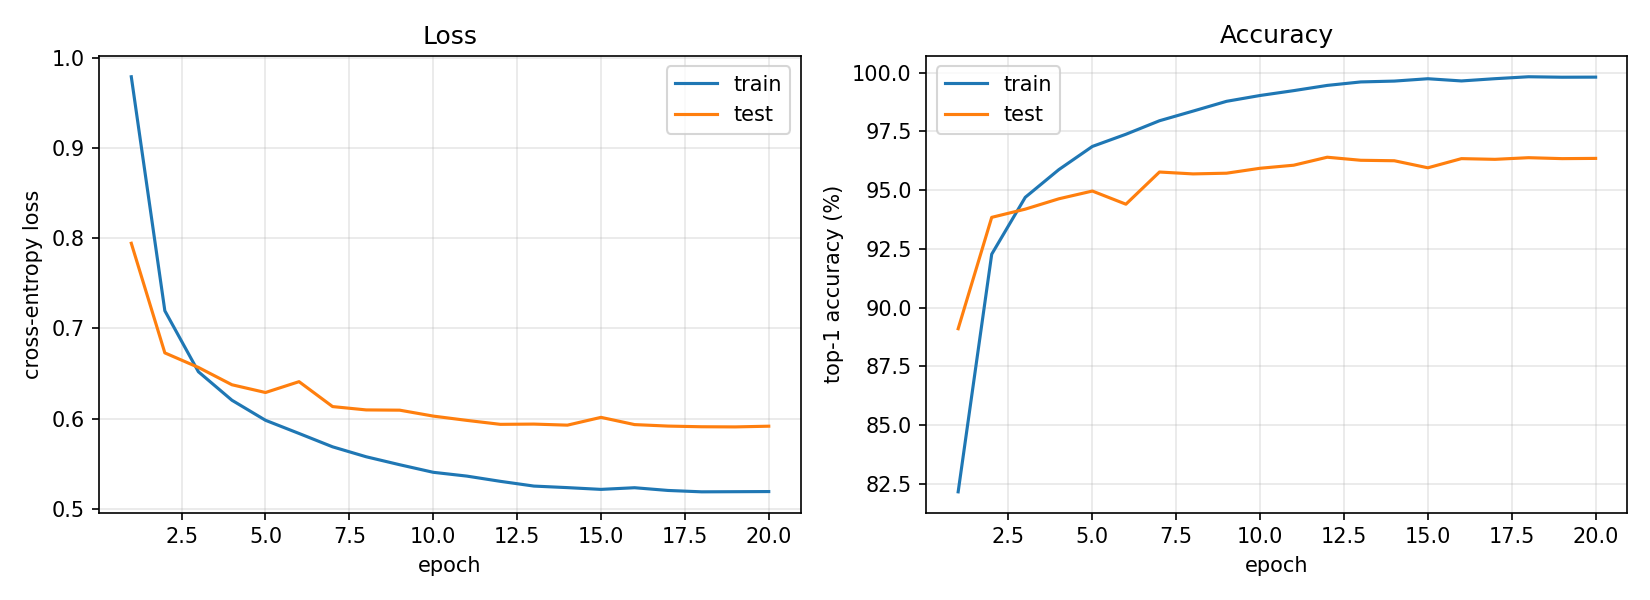
\includegraphics[width=0.85\textwidth]{figures/baseline_curves.png}
\caption{Training progress over 20 epochs.}
\label{fig:curves}
\end{figure}

The training accuracy gets very close to 100\%, but the test accuracy stops improving around epoch 12. This gap means the model is memorizing the data a bit. It shows the model is bigger than it needs to be for this simple dataset, which makes it a great choice for compression.

\paragraph{Where the Model Fails:} As shown in Table~\ref{tab:perclass}, the model mostly messes up on things that look alike.

\begin{table}[ht]
\centering
\begin{tabular}{@{}lcccccccccc@{}}
\toprule
Class & plane & auto & bird & \textbf{cat} & deer & \textbf{dog} & frog & horse & ship & truck \\
\midrule
Accuracy (\%) & 97.6 & 98.4 & 95.9 & \textbf{91.2} & 96.5 & \textbf{92.7} & 98.8 & 97.4 & 98.1 & 96.8 \\
\bottomrule
\end{tabular}
\caption{Test accuracy for each class.}
\label{tab:perclass}
\end{table}

Almost a quarter of all mistakes happen because it confuses cats and dogs (48 cats guessed as dogs, and 40 dogs guessed as cats). It also confuses trucks and cars 38 times. Since the original images are only $32\times32$, stretching them to $160\times160$ doesn't magically add lost details like fur textures. Because of this, the model has a hard time telling apart shapes that are very similar.

%======================================================================

\section{How Model is compressed}

\label{sec:compression}

%======================================================================

We shrink the model in three steps: removing useless weights (pruning), using smaller numbers (quantization), and packing the data tightly (Huffman coding).

\subsection{}

\paragraph{Pruning:} We remove weights that are closest to zero across the whole model at once. This works better than doing it layer by layer. To make sure no single layer gets completely destroyed, we cap the removal at 95\% per layer. We found that removing 50\% of the weights works well. If we try to remove 70\%, the model breaks and drops to 13\% accuracy.

\paragraph{Weight Quantization:} We change the main weights into simple integers (like 4-bit numbers) to save space. We test a few scaling options to find the one that causes the least error, which gives us about a 2\% boost in accuracy compared to the simplest method.

\paragraph{Activation Quantization:} We also shrink the outputs between the layers (activations) down to 8 bits. Instead of using the absolute maximum and minimum values to set our scale, we ignore the top 0.1\% of extreme values. This small change kept the accuracy at 95.85\%, whereas the basic method dropped it to 89.55\%.

\paragraph{Huffman Coding:} Since a lot of the weights become zero after pruning, we use Huffman coding. This is a lossless trick that gives short codes to common numbers (like zero) and longer codes to rare numbers. This saves an extra 15--35\% of space.

\subsection{Which Layers Matter Most?}

MobileNet-v2 is mostly made of two types of layers. The "pointwise" layers hold about 96.5\% of the model's parameters. The "depthwise" layers, along with the very first and last layers, hold only about 3.5\%.

\begin{table}[ht]
\centering
\begin{tabular}{@{}llrr@{}}
\toprule
\textbf{Layer} & \textbf{Type} & \textbf{Params} & \textbf{Acc. Drop at 3-bit} \\
\midrule
\texttt{features.1.conv.0.0} & depthwise & 288 & $-50.80\%$ \\
\texttt{features.3.conv.1.0} & depthwise & 1{,}296 & $-2.10\%$ \\
\texttt{features.14.conv.2} & pointwise & 92{,}160 & $-2.10\%$ \\
\texttt{features.17.conv.2} & pointwise & 307{,}200 & $-0.25\%$ \\
\texttt{features.18.0} & pointwise & 409{,}600 & $0.00\%$ \\
\bottomrule
\end{tabular}
\caption{How much accuracy drops if we compress just one layer to 3 bits.}
\label{tab:sensitivity}
\end{table}

As Table~\ref{tab:sensitivity} shows, if we squeeze a tiny depthwise layer down to 3 bits, the accuracy crashes by 50.80\%. But we can squeeze the massive pointwise layers and the accuracy barely moves. Because of this, we use a \textbf{mixed strategy}: we compress the big layers a lot (to 3 or 4 bits) and prune them. We leave the small, sensitive layers safely at 8 bits and don't prune them. This trick gave us a huge 14.4\% accuracy boost for almost no extra storage cost.

\subsection{Storage Details}

To report the real size, we have to count everything, including the scales and biases. As Table~\ref{tab:overhead} shows, we keep our scales in 16-bit float (FP16). Trying to squeeze scales down to 8 bits caused too many errors and ruined the model.

\begin{table}[ht]
\centering
\begin{tabular}{@{}lrr@{}}
\toprule
\textbf{Component} & \textbf{Size (KB)} & \textbf{Share} \\
\midrule
Main weights (Huffman) & 1012.5 & 91.4\% \\
Scales (FP16) & 33.3 & 3.0\% \\
Biases (FP16) & 33.3 & 3.0\% \\
Huffman dictionary & 4.9 & 0.4\% \\
\midrule
\textbf{Total} & \textbf{1049.2} & \textbf{100.0\%} \\
\bottomrule
\end{tabular}
\caption{Size breakdown for the basic 4-bit model without pruning.}
\label{tab:overhead}
\end{table}

%======================================================================

\section{Testing Different Settings}

\label{sec:q3}

%======================================================================

Before we spent time fine-tuning, we did a quick test to see how different bits and pruning levels behaved.

\begin{table}[ht]
\centering
\small
\begin{tabular}{@{}cccrrr@{}}
\toprule
\textbf{Main Bits} & \textbf{Output Bits} & \textbf{Sensitive Bits} & \textbf{Accuracy} & \textbf{Space Saved} & \textbf{Size (MB)} \\
\midrule
8 & 8 & 8 & 96.25\% & $4.2\times$ & 2.018 \\
8 & 8 & 4 & 81.21\% & $4.3\times$ & 1.981 \\
6 & 8 & 8 & 96.04\% & $5.6\times$ & 1.515 \\
6 & 8 & 4 & 77.26\% & $5.8\times$ & 1.478 \\
4 & 8 & 8 & 93.13\% & $8.1\times$ & 1.049 \\
4 & 8 & 4 & 62.64\% & $8.4\times$ & 1.012 \\
3 & 8 & 8 & 40.47\% & $10.3\times$ & 0.832 \\
3 & 8 & 4 & 17.87\% & $10.7\times$ & 0.794 \\
\bottomrule
\end{tabular}
\caption{Quick test of different bit sizes before fine-tuning.}
\label{tab:sweep}
\end{table}

\begin{figure}[ht]
\centering
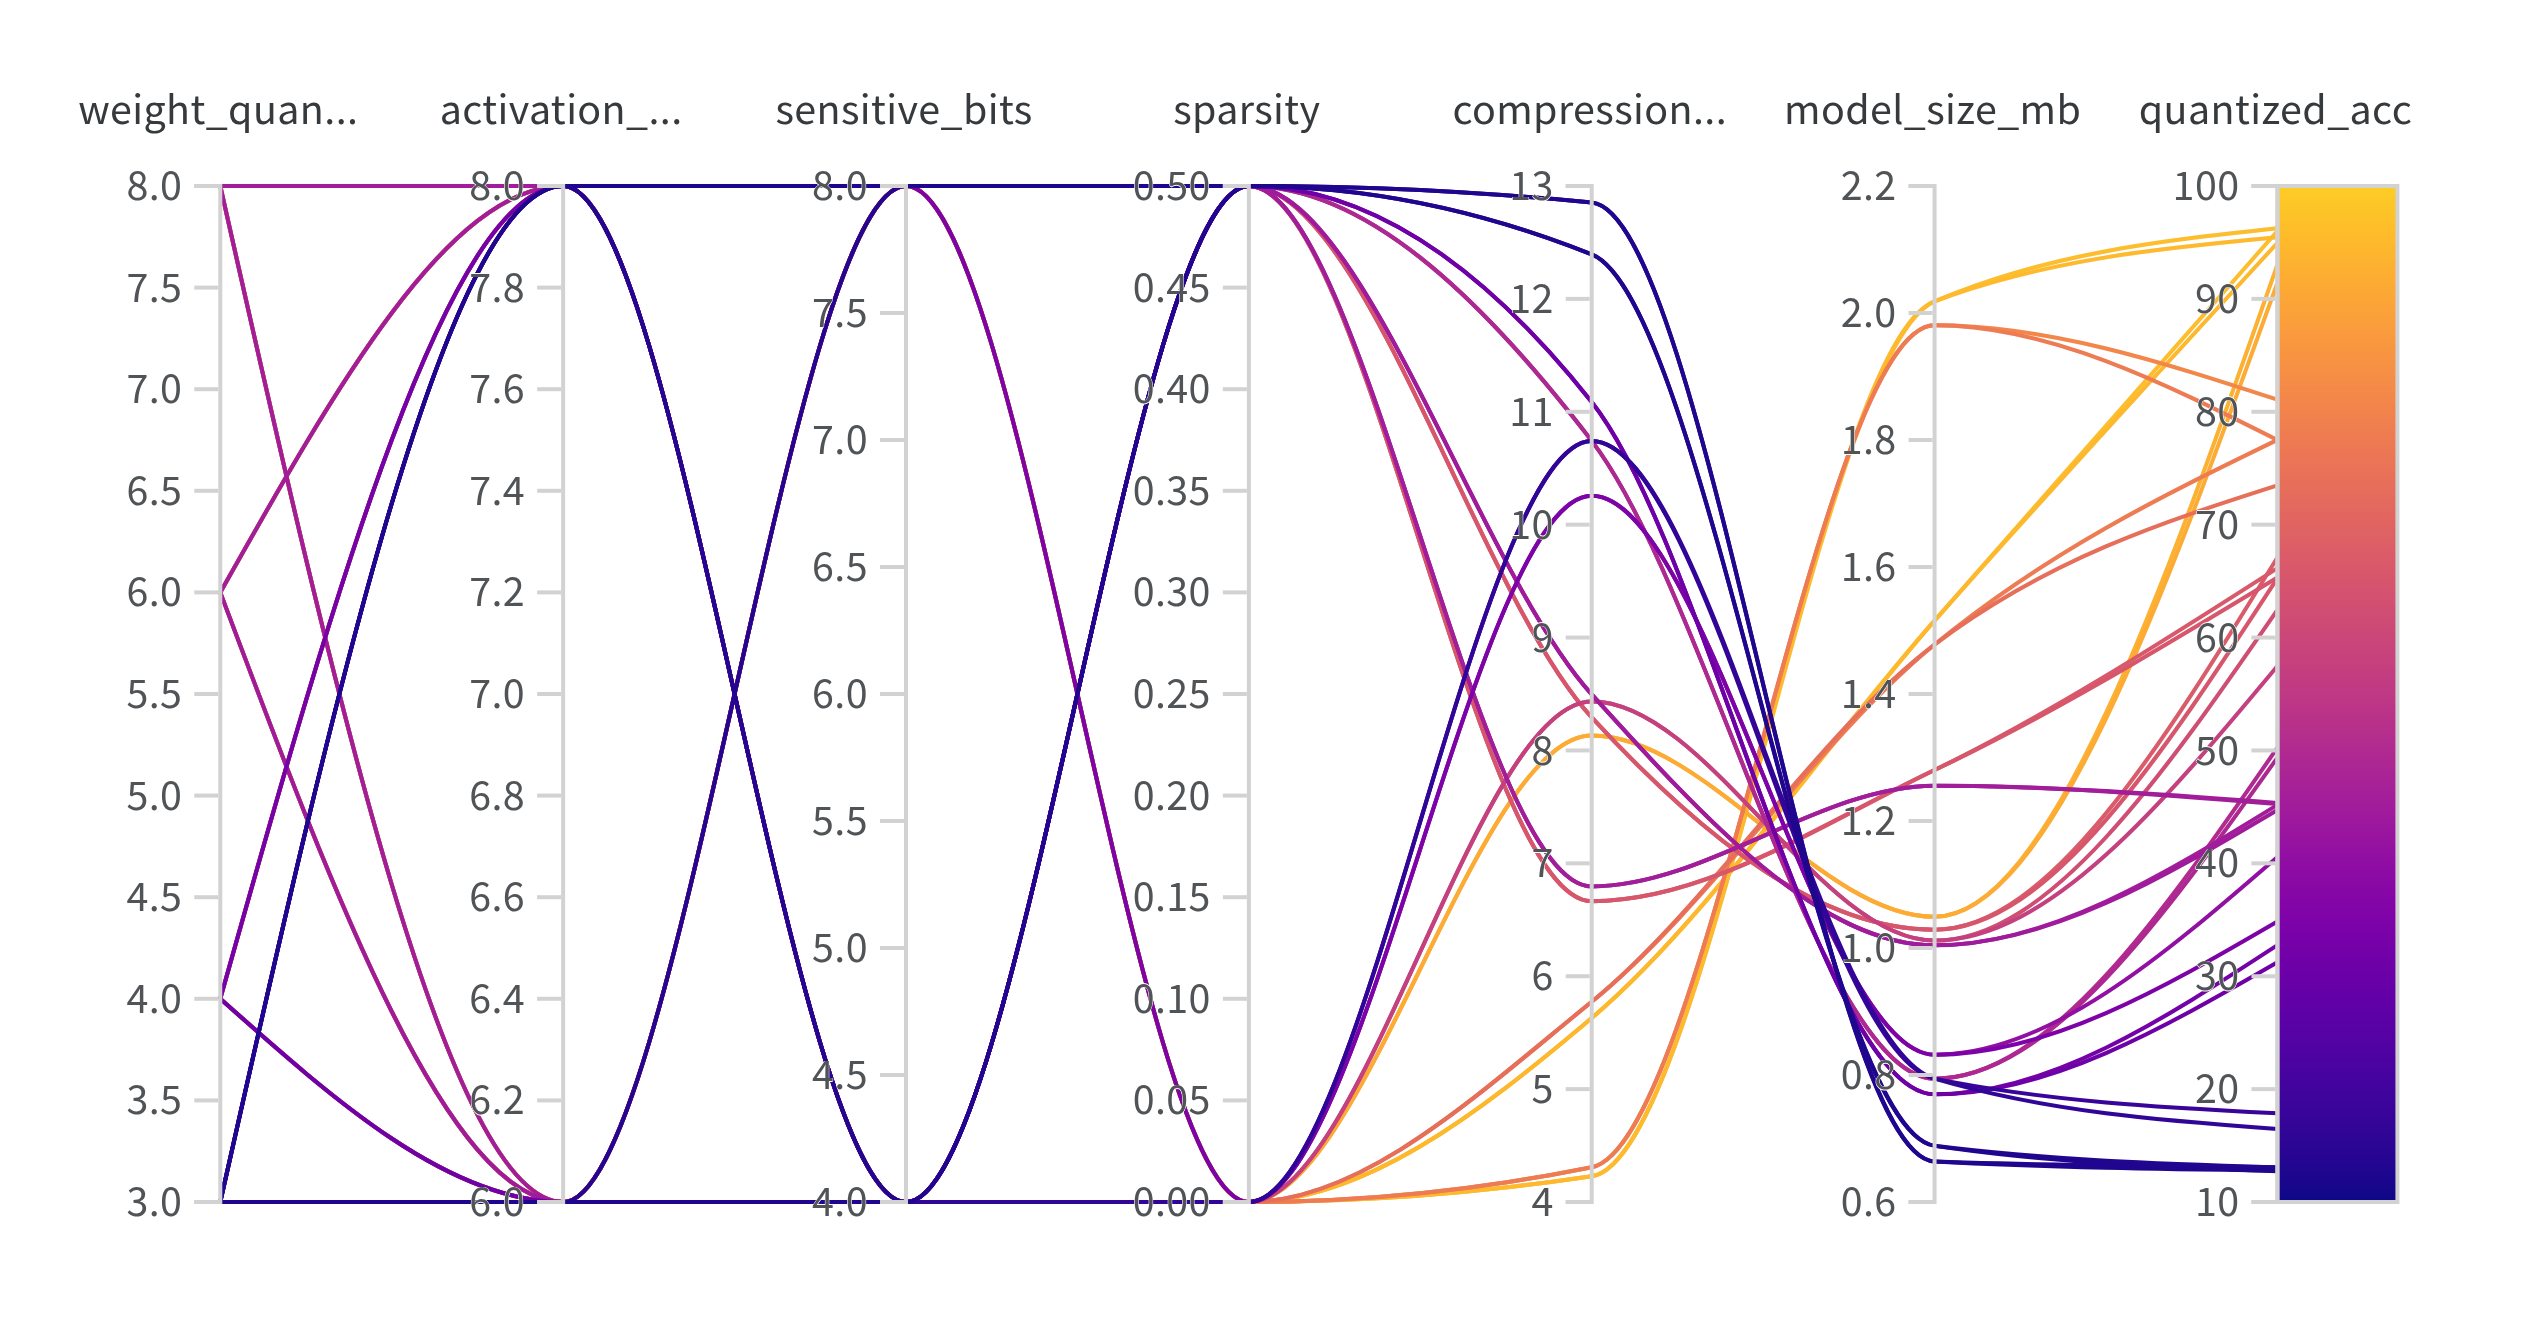
\includegraphics[width=0.95\textwidth]{figures/parallel_coordinates.png}
\caption{Chart of our 32 test runs. You can see the lines drop down (bad accuracy) whenever we try to compress the sensitive layers to 4 bits.}
\label{fig:parcoord}
\end{figure}

The main takeaway from Table~\ref{tab:sweep} and Figure~\ref{fig:parcoord} is that dropping the sensitive layers from 8 bits to 4 bits always destroys the accuracy. And since those layers are so small, squeezing them barely saves any space anyway. Keeping the sensitive layers at 8 bits is the most important rule we found.

%======================================================================

\section{Final Results}

\label{sec:q4}

%======================================================================

After picking our best setups, we trained them for 20 more epochs (fine-tuning) to recover the lost accuracy. Table~\ref{tab:candidates} shows the final numbers.

\begin{table}[ht]
\centering
\begin{tabular}{@{}lrr@{}}
\toprule
\textbf{Configuration} & \textbf{Accuracy} & \textbf{Space Saved} \\
\midrule
4-bit (no pruning) & 94.97\% & $8.13\times$ \\
Mixed bits (no pruning) & 93.74\% & $9.43\times$ \\
3-bit (no pruning) & 93.10\% & $9.91\times$ \\
\textbf{4-bit + 50\% pruning (chosen)} & \textbf{93.23\%} & \textbf{$10.74\times$} \\
\bottomrule
\end{tabular}
\caption{Final accuracy after fine-tuning.}
\label{tab:candidates}
\end{table}

Our absolute best model uses \textbf{50\% pruning} on the big layers, combined with \textbf{4-bit weights}, \textbf{8-bit activations}, and \textbf{Huffman coding}:

\begin{itemize}

\item \textbf{(a) Weight Compression:} The weights take up $\mathbf{11.03\times}$ less space compared to the original model.

\item \textbf{(b) Activation Compression:} The data moving between layers takes up $\mathbf{4.0\times}$ less space (shrunk from 32-bit floats to 8-bit integers).

\item \textbf{(c) Accuracy:} It reached \textbf{93.23\%}. This means we only lost about 3.11\% accuracy compared to the original model, which is a great trade-off.

\item \textbf{(d) Final Size:} The total file size is just $\mathbf{0.795\text{ MB}}$ ($\mathbf{813.6\text{ KB}}$), down from $8.53$~MB.

\end{itemize}

\begin{table}[ht]
\centering
\begin{tabular}{@{}lrr@{}}
\toprule
\textbf{Component} & \textbf{Size (KB)} & \textbf{Share} \\
\midrule
Main weights (Huffman) & 742.5 & 91.3\% \\
Scales (FP16) & 33.3 & 4.1\% \\
Biases (FP16) & 33.3 & 4.1\% \\
Huffman dictionary & 4.5 & 0.5\% \\
\midrule
\textbf{Total Size} & \textbf{813.6} & \textbf{100.0\%} \\
\bottomrule
\end{tabular}
\caption{Final size breakdown of our best compressed model.}
\label{tab:overhead-final}
\end{table}

\end{document}
